\chapter{Event reconstruction}
\label{ch:reconstruction}

As described in Chapter~\ref{ch:lhcAndCMS}, the CMS detector
is built from complementary detector components with sensitivity
to stable particles: electrons, muons, photons, and charged
and neutral hadrons. Each can be distinguished by the likelihood of interaction
and interaction characteristics with the detector components:
all charged particles leave tracks in the tracker,
charged hadrons deposit energy in the calorimeters, photons
and electrons primarily deposite energy in the ECAL, and neutral
hadrons interact primarily with the HCAL.
The reality is more subtle than this idealized picture, illustrated
in Fig.~\ref{fig:particleFlow}, but this forms the guiding principles
in the \emph{reconstruction} of particles from their interactions in the detector.
Unstable particles are inferred by the properties of the stable particles to 
which they decay.

\begin{figure}[htbp]
  \centering
   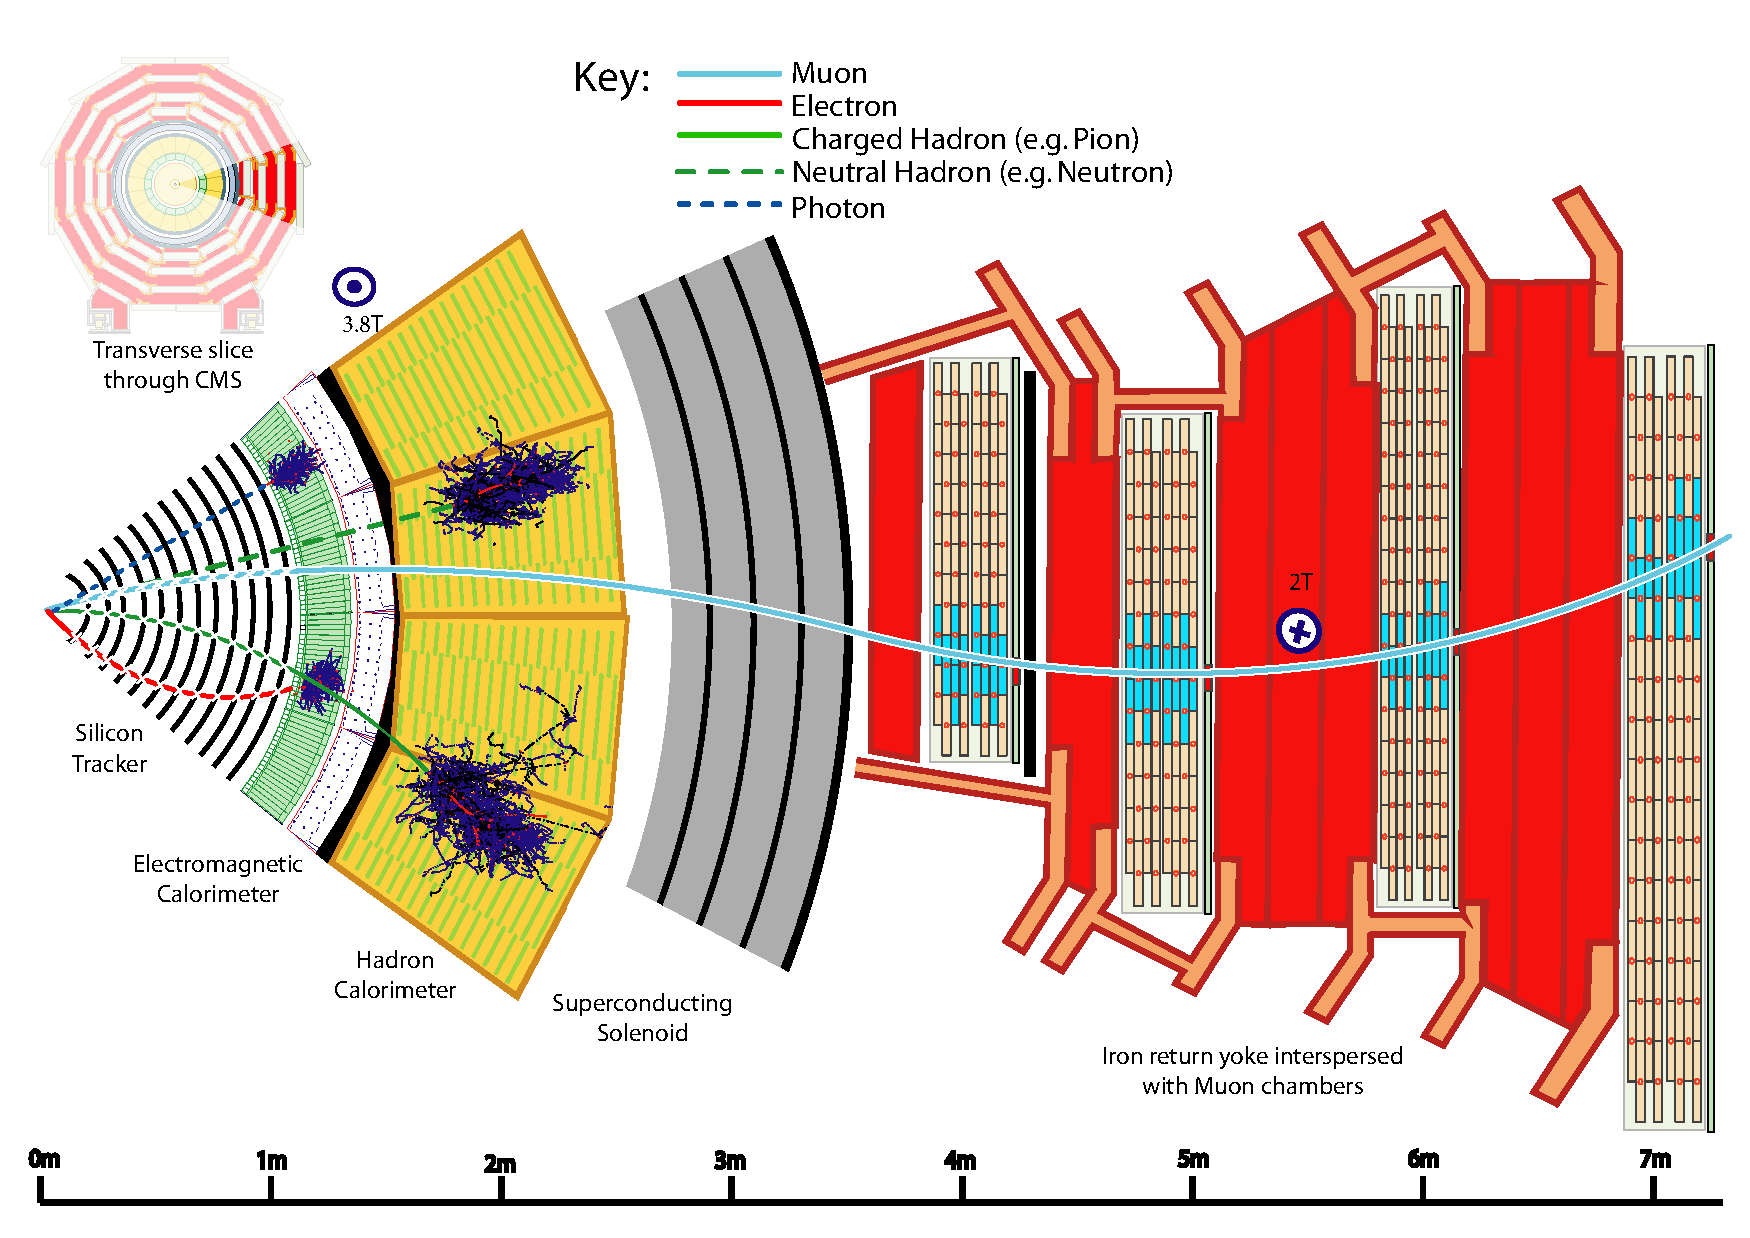
\includegraphics[width=\textwidth]{figures/Reconstruction/CMSDetectorParticleFlow.pdf}
  \caption{
    Idealized picture of particle interactions with the CMS detector subsystems.
        }
 \label{fig:particleFlow}
\end{figure}

When an event is accepted by the HLT, the raw, digitized data from each detector
subsystem is stored and simultaneously forwarded to a commercial processing farm for
further processing. Detector-specific attributes, such as signal amplitudes,
are converted to physical properties, such as energies, using calibrations
established from controlled independent measurements. System-wide patterns
are built, from which a global picture of the event and its component particles
are inferred.
The reconstruction algorithms employed by the CMS Collaboration are built from
work that began well before the LHC began taking data, 
benefiting from generations of previous experiments. The development of algorithms
is an iterative process, with continual optimizations and incremental changes
being made. The techniques described here relate to the data collection and reconstruction
used by the CMS Collaboration in 2016. Many aspects of the reconstruction
are shared by all analyses performed by the CMS Collaboration. 

A degree of ambiguity in particle identification is unavoidable. 
Reconstruction \emph{efficiency}, or a high rate of positive identification
and reconstruction of real particles, must be balanced alongside the rate of misconstruction.
For example, electrons with a poorly reconstructed track will mimic photons,
but because the track reconstruction efficiency cannot be 
accepting only very high-quality tracks will lead to a lower rate 
of indentification 
The optimal balance between efficiency and misidentification is dependent
on the characteristics of the signal and background targeted by a particular
analysis. In addition to the common reconstruction features, the identification 
criteria used in this work are also discussed.


\section{Global event description via particle flow}
The general characteristics of physics object identification outlined
above are ubiquitous amongst past, current, and future collider detector
reconstruction algorithms. Rather than applying these criteria object by
object, the CMS Collaboration exploits the 

By applying these characteristics

\subsection{Tracks and vertices}
Only energy deposits from charged particles traversing the pixel detector and
strip tracker that exceed a threshold energy (adjustable for each element)
are retained for offline storage. The position of each \emph{hit} is locally
reconstructed from clusters of adjacent pixel or strip elements based
on the relative collected charge in the cluster. 
The efficiency for hits to be reconstructed is over 99\% for active 
channels in both the pixel and strip detectors; approximately 98\%
of pixel channels and 96\% of strip channels were active during 2016 data collection.
The hit position is calculated
in local coordinates of the detector elements before being converted
into a global position with respect to the full CMS detector. The transformation
to global coordinates depends on the relative alignment of the individual tracker
elements and their alignment with respect to the other detector systems.
This is established through in situ measurements of the paths of cosmic rays
to an uncertainty neglible with respect to the intrinsic position resolution 
of the silicon detectors~\cite{Chatrchyan:2014wfa}.

The paths of charged particles through the detector are derived by 
fitting curves to the hits along a possible trajectory. 
The high combinatorics of possible track patterns that can be derived
from the large number of hits arising from high-particle-multiplicity
events is a computational challenge.
To reduce the complexity of pattern identification
while maintaining a high efficiency of reconstruction, the tracking finding
algorithm proceeds in steps, designed to first identify unambiguous
tracks before recovery those of lower quality.
Hits used to form tracks in are removed from consideration in the following
steps, reducing the complexity and chance for misassociation.

In all steps, the algorithm begins with an initial projection of the track
direction, referred to as the track \emph{seed}. The track is then formed
sequentially by extrapolating outward from the beam interaction---in the 
case of tracks seeded by the inner tracker, or inward from seeds in the muon
chambers of calorimeter clusters. Subsequent hits are located 
by predicting their location with using the
Combinatorial Track Finder (CTF) alogrithm~\cite{Chatrchyan:2014fea}, 
an adaptation of the combinatorial Kalman filter algorithm~\cite{}. 
At each step, the projected trajectory is updated to account for the additional
associated seeds, simultaneously building and fitting the particle path.
When the full trajectory through the tracker is established, the track
is refit and discarded if it fails to meet quality criteria, such as 
an excessively high $\chi^{2}$ of the fit.

The first track-forming iterations target high-quality, high-$\pt$ tracks associated
with the beam crossing region, or \emph{beam spot}, established over many
collisions by fitting the expected Gaussian beam profile to the observed
pixel tracks. These initial iterations use seeds formed from hits in each layer of 
the pixel detector, relaxed to two hits in subsequent iterations. 
Following iterations relax the requirement for the track seed to be
compatible with the beam spot, instead seeding via successive hits in the strip
tracker, increasing sensitivity
to displaced tracks from heavy-flavor hadron decays. 
Final iterations are seeded by the muon detectors using an outside-in approach.

Electrons traveling through the tracker have up to $\approx$85\% probability 
of radiating photons (known as bremsstrahlung)
due to interactions with the significant tracker material. Therefore, electron
tracks are likely to exhibit sharp kinks from sudden energy loss by bremsstrahlung.
A modified algorithm known as Gaussian sum filter (GSF)~\cite{Adam:2005bya} is thus employed to 
more accurately reconstruct electron-like tracks. In the CTF algorithm, the
Kalman filter accounts for the material interactions with a Gaussian
smearing around the expected hit location. In the GSF algorithm, 
a sum of Guassian terms, designed to reproduce the Bethe formula for electron
energy loss~\cite{doi:10.1098/rspa.1934.0140}, is used. The GSF algorithm is applied to a subset of 
tracks formed via the CTF algorithm that have few associated hits or a relatively
poor $\chi^{2}$ to obtain an improved description under the electron hypothesis.
The GSF algorithm is also used to form tracks seeded by energy clusters in the 
ECAL, described in Section~\ref{sec:ereco}.

Because the collisions analyzed for this work generally involve multiple $\pp$ interactions,
tracks originate from a variety or vertices. Vertices 
associated with a $\pp$ collision and not an interaction or decay displaced from
the collision point are identified by evaluating the common points of origin for a subset
of the track collection that are well-reconstructed (low $\chi^{2}$) and consistent with
the beam spot. No additional condition on the track $\pt$ is applied
to select this reduced track collection. The deterministic
annealing algorithm~\cite{} is used to group the tracks into their most probably set
of common vertices, before the vertex coordinates are derived by a fit to the 
associated tracks, considering their likelihood of misassignment to the vertex.

The \emph{primary vertex} is the vertex associated with the hard scattering interaction
of interest. The vertex that maximizes $\sum_{i}\pt^{2}$, where the sum considers
the tracks associated with the vertex---clustered using the anti-\kt algorithm
described in Section~\ref{sec:jreco} with radius parameter $R=0.4$---and the 
transverse momentum imbalance associated with the vertex and clustered tracks.
Studies of simulated $\WZ$ events demonstrate that this approach selects the
correct $\pp$ vertex more than 99\% of the time for signal processes considered here. 

\subsection{Calorimeter clusters}
Energy deposits in the calorimeter are the other crucial component of particle
identification and reconstruction in the CMS detector.

Calorimeter clusters are 
\subsection{Particle flow candidates}

\section{Physics objects}
  \subsection{Muons}
  Talk about PF muons
  global vs. tracker


\subsection{Electrons}
\label{sec:ereco}

\begin{table}[htbp]
    \centering
    \caption[]{
            }
    \begin{tabular}{lccc} 
    Variable  & Loose ID  & Tight ID \\
    \hline 

    
     \end{tabular}
    \label{tab:control_regions}
\end{table}
  \subsection{Charged and neutral hadrons}
  \subsection{Jets}
  \subsection{Identification b-jets}
  \subsection{Missing transverse momentum}

